% \tdi{Voir comment citer les 2 naive physics manifestos}

\subsection{Éléments généraux sur la localisation par référencement
  indirect et formalisation d'une relation de localisation}

\subsubsection{Les concepts de \emph{sujet} et \emph{d'objet de
    référence}}

% Mise au point vocabulaire
Comme nous l'expliquions précédemment (\autoref{subsec:2-1}) un
\emph{indice de localisation} est composé de trois éléments :
%
\begin{enumerate*}[label=(\alph*)]
\item \label{i:site} un \emph{sujet,}
\item \label{i:cible} un \emph{objet de référence} et
\item une \emph{relation de localisation,}
\end{enumerate*}
%
qui, combinés, permettent d'exprimer un \emph{référencement indirect.}
Ainsi, on peut trouver ces trois éléments dans des phrases aussi
variées que : \textquote[{\cite[79]{Borillo1998}}]{l'extérieur de la
  boîte est laqué}, \textquote[{\cite[101]{Vandeloise1986}}]{la
  chaumière est au-dessus de la tour} ou \enquote{le chalet est à une
  heure de marche}. Cette décomposition ternaire semble faire l'objet
d'un consensus scientifique, puisqu'elle est partagée par toutes les
formalisations des \emph{référencements spatiaux indirects} que nous
avons rencontrés.

Les différences entre ces travaux portent avant tout sur le
vocabulaire employé pour nommer ces concepts et dont
\textcite{RetzSchmidt1988} a proposé une synthèse. Le vocabulaire
varie bien évidement en fonction de la langue de publication, mais
également en fonction de la discipline des auteurs. En linguistique
francophone \autocite{Vandeloise1986,Borillo1998, Aurnague1997,
  Mathet2000}, par exemple, les termes de \emph{site} et de
\emph{cible} sont employés pour désigner, respectivement,
\emph{l'objet de référence} et le \emph{sujet.}
%
La littérature anglophone abonde de termes pour désigner ces deux
concepts, comme \emph{primary object} et \emph{reference object}
employés par \textcite{RetzSchmidt1988, Clementini2013}, \emph{figure}
et \emph{ground} utilisés par \textcite{Talmy1983} ou encore
\emph{trajector} et \emph{landmark,} qui sont la utilisée par
\textcite{Vandeloise1984} des termes \emph{site} et \emph{cible.}
%
Mais sous cette grande disparité de vocabulaire se cachent en réalité
les deux mêmes concepts.

%TODO
%\tdi{Faut-il plus détails ?}

\subsubsection{\emph{Relations spatiales et relations de localisation}}

Comme pour les termes de \emph{sujet} et \emph{d'objet de référence,}
différents termes sont utilisés comme synonymes de
\enquote{\emph{relation de localisation}}, comme
\enquote{\emph{relation spatiale}}, qui est le terme le plus
fréquemment utilisé. Toutefois, contrairement aux différents synonymes
de \emph{sujet} et \emph{d'objet de référence}, les termes de
\emph{relation spatiale} et de \emph{relation de localisation} ne sont
pas nécessairement considérés comme
équivalents. \textcite{Duchene2019}, par exemple, font la distinction
entre les \emph{relations spatiales,} qui sont énoncées avec une
préposition spatiale (\eg \emph{sur, sous, dans, à côté,} etc.) et les
\emph{relations de localisation} qui décrivent une position sans
nécessairement faire appel à une \emph{préposition spatiale}, comme
dans les phrases : \enquote{Je suis à cinq minutes de marche} ou
\enquote{Je vois un chalet}. Cependant, cette distinction est souvent
occultée. Pour \textcite{Vandeloise1986}, toute relation décrivant une
position, avec ou sans \emph{préposition spatiale,} est une
\emph{relation spatiale.} De son point de vue, la sémantique prime
donc sur la morphologie.

De plus, dans les travaux de \textcite{Bateman2010}, les relations
décrivant l'organisation spatiale d'un groupe (\eg \enquote{être
  alignés}) sont considérés comme des \emph{relations spatiales,} bien
que ne décrivant pas une position. Si l'on accepte de qualifier ces
relations, décrivant une organisation intra-groupe, comme des
\emph{relations spatiales} alors on ne peut pas considérer que
l'ensemble des \emph{relations spatiales} est inclus dans l'ensemble
des \emph{relations de localisation,} \ie que toute \emph{relation
  spatiale} et une \emph{relation de localisation.}

Nous pourrions donc utiliser exclusivement le terme de \emph{relation
  spatiale.} Cependant, le vocabulaire proposé par
\textcite{Duchene2019} permet de distinguer les relations susceptibles
d'être \emph{spatialisées}, \ie les \emph{relations de localisation}
des \emph{relations spatiales,} qui, si l'on intègre les
configurations intra-groupe, comme le propose \textcite{Bateman2010},
ne le sont pas nécessairement. Ainsi, dans la suite de ce travail nous
parlerons exclusivement de \emph{relations de localisation.}

Contrairement à ce que pourraient laisser penser les différents
exemples \emph{d'indices de localisation} présentés jusqu'ici, ces
derniers peuvent contenir plus d'un \emph{objet de référence}
\autocite{Clementini2013}. Ce cas, moins fréquent, se présente lorsque
la \emph{relation de localisation} utilisée n'est pas \emph{binaire,}
c'est-à-dire qu'elle n'implique pas qu'un \emph{sujet} et qu'un
\emph{objet de référence.} Le cas le plus fréquent est celui de la
\emph{relation de localisation} \enquote{entre} qui implique, au
minimum, deux \emph{objets de référence.} On parle alors de
\emph{relation de localisation ternaire}. En effet, si l'on peut dire
que \enquote{La poste est entre le café et la banque}, il est
incorrect d'utiliser cette \emph{relation de localisation} avec un
seul \emph{objet de référence.} La phrase \enquote{Je suis entre
  l'université}, par exemple, est fautive et incompréhensible.

Cependant, tous les \emph{indices de localisation} composés de trois
objets, n'impliquent pas nécessairement une \emph{relation de
  localisation ternaire} \autocite{Duchene2019}. L'un des objets peut,
par exemple, être le support des deux autres, c'est par exemple le cas
lorsqu'une position est décrite sur un itinéraire, comme dans la
phrase \enquote{le parking est avant le pont}. De même, une phrase
comme : \enquote{Il est à l'angle de la rue Saint-Jacques et de la rue
  Pierre et Marie Curie}, qui contient trois objets spatiaux :
\emph{le sujet} (\enquote{Il}) et deux objets de référence
(\enquote{rue Saint-Jacques} et \enquote{rue Pierre et Marie Curie}),
ne contient pas de \emph{relation de localisation ternaire}. Dans ces
deux cas, on peut recombiner l'énoncé en un ensemble \emph{d'indices
  de localisation} utilisant des \emph{relations de localisation
  binaires.} Par exemple, \enquote{l'angle de la rue Saint-Jacques et
  de la rue Pierre et Marie Curie} peut être considéré comme un seul
\emph{objet de référence,} cette description de position peut
s'interpréter comme deux \emph{indices de localisation :} \enquote{Je
  suis à un endroit et cet endroit est à l'intersection de la rue
  Saint-Jacques et de la rue Pierre et Marie Curie}. Ces exemples
n’intègrent donc pas de \emph{relations de localisation ternaires.} À
l'inverse, des phrases ne contenant qu'un seul \emph{objet de
  référence} peuvent utiliser des \emph{relations de localisation
  ternaires.} On pourra par exemple dire : \enquote{La vache est entre
  les arbres}, dans ce cas, seul un \emph{objet de référence,}
\enquote{les arbres}, est présent, mais celui-ci est composite.
\textcite{Aurnague1993} parlent alors de \enquote{\emph{collection}}.


\subsubsection{Contexte d'interprétation et cadre de référence}

% \tdi{citer Spatial representation and updating: Evidence from
%  neuropsychological investigations}

% \tdi{citer The Role of Context in the Interpretation of Natural
%   Language Location Descriptions}

Comme les différents exemples utilisés jusqu'ici le laissent supposer,
certaines \emph{relations de localisation} ne peuvent être
interprétées ---~et donc \emph{spatialisées}~--- sans une connaissance
supplémentaire sur la configuration de la position décrite. C'est par
exemple le cas dans des phrases telles que : \enquote{Elle est devant
  l'université} ou \enquote{La poste est à gauche}. Les
\emph{relations de localisation} \enquote{devant} et \enquote{à
  gauche} ont une signification dépendante du contexte.

Notre gauche et notre droite sont dépendantes de notre orientation et
le \enquote{devant} de notre sens de déplacement
\autocite{Vandeloise1986}. On pourra facilement se convaincre qu'il
est illusoire d'interpréter ces \emph{relations de localisation} sans
une connaissance exogène, un \emph{référentiel de directions} (ou
\emph{cadre de référence,} selon \cite{Clementini2013}). Pour
reprendre l'exemple de l'indice de localisation : \enquote{Elle est
  devant l'université}, on peut l'interpréter de deux manières
différentes. Si le \emph{cadre de référence} est l'université, alors
on considèrera que son \enquote{devant} est la face où se situe
l'entrée principale. Alors que si la référence est un observateur
externe on pourra considérer que n'importe quelle positon située entre
l'observateur et l'université sera \enquote{devant}, car avec ce
second référentiel, l'orientation du locuteur sert de référence. Les
\emph{relations de localisation} dont l'interprétation nécessite un
\emph{cadre de référence} sont généralement qualifiées de
\emph{projectives} et \emph{directionnelles} \autocite{Duchene2019}.

L'interprétation de ces \emph{relations de localisation} est
compliquée par le fait que le \emph{cadre de référence} ne soit pas
nécessairement explicité dans \emph{l'indice de localisation,} comme
dans l'exemple précédent, \enquote{Elle est devant l'université},
alors qu'il l'est dans la phrase \enquote{il est à ma
  gauche}. L'article défini \enquote{ma} indique que le locuteur
utilise sa ligne de vue comme référence.

\subsubsection{Modélisation formelle d'un \emph{indice de localisation}}

Dans leur ontologie, \textcite{Bateman2010} définissent les notions
\emph{d'objet} (qui peut être localisé) et de \emph{place} (le lieu où
un \emph{objet} peut être localisé). La particularité des
\emph{places} est qu'elles peuvent êtres définies à partir d'un
\emph{objet de référence,} ce qui permet la modélisation
\emph{d'indices de localisation récursifs,} comme dans la phrase
\enquote{À gauche de l'ordinateur il y a une clé USB}, tirée de
\textcite{Bateman2010}. On retrouve dans cet exemple deux
\emph{indices de localisation distincts.} Le premier, décrit la
position d'une clé USB à partir d'un \emph{objet de référence} (ou
\emph{place} selon le vocabulaire de \textcite{Bateman2010} dont la
position est définie par un second \emph{indice de localisation.} Dans
cette ontologie, le lieu \enquote{À gauche de l'ordinateur} est
qualifié de \emph{GeneralizedLocalisation}. Cet objet est lui-même
composé de deux parties, la \emph{SpatialModality,} qui correspond à
ce que nous appelons \emph{relation de localisation} (\emph{À gauche
  de}) et le \emph{relatum,} ou \emph{objet de référence} selon notre
vocabulaire (\emph{l'ordinateur}). On peut remarquer que cette
ontologie conserve la structure en trois éléments distincts
(\emph{objet à localiser,} \emph{objet de référence} et \emph{relation
  de localisation}) que nous avions déjà présentés. C'est une
caractéristique également partagée avec la formalisation des
\emph{indices de localisation} proposée par \textcite{Vasardani2013},
dans le but de construire des croquis de situations à partir de
descriptions textuelles de positions. \textcite{Vasardani2013}
proposent de représenter les \emph{indices de localisation} par des
\emph{triplets,} de la forme : \(\langle L, r, R_o\rangle\) où \(L\)
est l'objet à localiser, \(r\) la \emph{relation de localisation} et
\(R_o\) \emph{l'objet de référence.} Par exemple, la phrase
\enquote{Je suis à côté d'une pizzeria} sera formalisée de la manière
suivante :
\(\langle \text{Je},\ \text{à côté},\ \text{pizzeria} \rangle\). Ce
formalisme en triplets est ensuite utilisé pour définir un graphe,
dont les objets spatiaux (\ie le \(L\) et le \(R_o\) d'un triplet)
sont les nœuds et la \emph{relation de localisation} les arêtes
orientées. Cette formalisation permet, comme dans l'ontologie de
\textcite{Bateman2010} de définir des indices de localisation
récursifs.

Comme le modèle de \textcite{Vasardani2013}, le modèle normalisé
ISO-Space, proposé par \textcite{Pustejovsky2017}, a pour objectif de
faire le lien entre une description de position textuelle et sa
représentation spatiale. Ce modèle est cependant beaucoup plus
détaillé que la proposition de \textcite{Vasardani2013}. D'une part,
car le modèle ISO-Space offre la possibilité de modéliser des
déplacements, d'autre part, il est construit au dessus de l'ontologie
de \textcite{Bateman2010}. Ainsi, certains concepts, comme la
\emph{spatial entity} (qui est l'objet à localiser) sont directement
repris de GUM-Space.

D'autres formalisations des \emph{relations de localisation} ont été
proposées dans le domaine de la géomatique, plusieurs travaux
nécessitant l'interprétation de \emph{relations de localisation.}
C'est par exemple le cas de la généralisation automatique, dont
l'objectif est de simplifier l'information cartographiée, tout en
conservant les relations géographiques entre objets. Par exemple, si
l'on simplifie la géométrie d'une rue il est souhaitable que les
bâtiments qui la longent, longent également la rue simplifiée. Ainsi,
même si la donnée cartographiée ne correspond pas parfaitement à la
réalité elle en conserve une caractéristique importante, les bâtiments
sont alignés le long de la rue. Pour ce faire, il est nécessaire
d'expliciter ces relations entre objets
cartographiés. \textcite{Duchene2004,Gaffuri2008} proposent, par
exemple, de représenter ces relations sous la forme d'objets portant
des contraintes quant à leur localisation. Quant à
\textcite{Touya2012}, ils proposent une ontologie permettant de
représenter les \emph{relations de localisation} entre objets
cartographiques, mais également les méthodes permettant de vérifier
ces relations.

Toujours dans le domaine de la généralisation cartographique,
\textcite{Jaara2012} ont proposé un modèle permettant d'exprimer les
\emph{relations de localisation} entre des objets géographiques, liés
à une base de données et des objets thématiques qui s'y
positionnent. Par exemple, un accident de la route est un objet
thématique, lié à un objet géographique, le réseau routier. La
modélisation de ces relations permet de conserver un lien cohérent
entre ces deux types d'objets lors du changement des objets
géographiques, par exemple lors du passage à un autre niveau de
détail. Comme dans les travaux de \textcite{Duchene2004,Gaffuri2008,
  Touya2012}, ce modèle permet donc d'exprimer des relations entre
objets que l'on veut voir conservées lors d'une modification. Bien que
traitant de \emph{relations de localisation,} ces travaux adoptent une
modélisation très centrée sur leur domaine
d’application. \textcite{Jaara2012} identifient, par exemple, deux
types d'objets, les \emph{objets supports} et les \emph{objets
  thématiques.} Bien que pouvant tous deux jouer le rôle de
\emph{sujet} ou \emph{d'objet de référence,} ils ne sont pas
distingués selon ce critère, mais en fonction de leur nature, ce qui
rend ce modèle assez différent de ce que proposent
\textcite{Bateman2010,Pustejovsky2017}.

Dans un domaine d’application assez différent, l'ontologie FRSO
\autocite{Hudelot2008a} propose une formalisation des \emph{indices de
  localisation} destinée à la segmentation automatique d'images
médicales. Les positions relatives des organes humains étant connues a
priori, la formalisation de cette connaissance permet d'ajouter des
connaissances exogène lors de la segmentation automatisée des
images. Une des particularités de l'ontologie de
\textcite{Hudelot2008a} est qu'elle définir un concpet,
\emph{ReferenceSystem,} qui permet de définir un \emph{cadre de
  référence.}

Enfin, \textcite{Trinh2012} propose un modèle permettant de formaliser
des \emph{relations de localisations} entre objets au sein d'une scène
3D. Comme dans l'ontologie FRSO, les \emph{relations de localisation}
sont modélisées comme des concepts et non comme des relations. Ce
modèle propose également la prise en compte de la notion de
\emph{cadre de référence,} sauf que, contrairement à la proposition
d'\textcite{Hudelot2008a}, deux cadres de référence distincts sont
définis : le premier défini implicitement et un second défini
explicitement, lorsque les contraintes modélisées impliquent la
présence d'un observateur.

Pour conclure sur ces différentes formalisation des \emph{indices de
  localisation,} on peut remarquer, comme le signale
\textcite{Duchene2019}, deux point essentiels. Le premier est celui
qui consiste à modéliser les \emph{relations de localisation} comme
des concepts, ce qui par ailleurs la solution majoritairement
retenue. Le second point est que la notion de \emph{cadre de
  référence} est rarement modélisée alors que, comme nous
l'expliquions précédemment, elle est indispensable à l'interprétation
de certaines \emph{relations de localisation.}

\subsection{Classification et ontologies des \emph{relations de
    localisation}}

Plusieurs catégories de \emph{relations de localisation} peuvent êtres
définies. On peut par exemple distinguer celles qui sont exprimées à
l'aide d'une \emph{préposition spatiale} (\ie les relations spatiales)
et celles qui ne le sont pas. Mais, on peut également utiliser
d'autres critères, par exemple sémantiques ou morphologiques. De
nombreux travaux ont cherché à catégoriser les \emph{relations de
  localisation} en fonction de ces critères (ou d'autres) à la fois
pour en faciliter la compréhension, pour mettre en évidence des
similarités ou des redondances, mais également dans le but d'appliquer
ces classifications à des cas concrets, comme la \emph{spatialisation
  d'indices de localisation.} Nous allons présenter ces différentes
classifications proposées dans la littérature et ce à l'aide d'une
démarche en deux étapes. Dans un premier temps, nous présenterons les
différentes classifications des \emph{relations de localisation}
proposées dans la littérature, puis nous nous focaliserons sur une
catégorie particulière de classification, les \emph{ontologies,} qui
formalisent ces classifications.

\subsubsection{Classification des \emph{relations de localisation}}

La classification de \emph{relations de localisation} nécessite de
définir un ensemble de critères de catégorisation. La majorité des
catégorisations de \emph{relations de localisation} que nous avons
rencontrées utilisent un seul critère, par exemple la
\emph{sémantique,} ou le\emph{ niveau d'astraction.} Mais on trouve
également des organisations \enquote{hybrides}, qui combinent
plusieurs critères.

Le choix de ce critère nous semble fortement lié au domaine
d’application de la classification et plus encore à sa discipline de
rattachement. En linguistique, par exemple, les classifications sont
généralement organisées suivant un critère sémantique. Par exemple, on
distinguera les \emph{relations de localisation} traduisant un
mouvement, de celles décrivant une position fixe
\autocite{Borillo1998}. À l'inverse, les classifications réalisées
dans des domaines se rattachant à l'informatique et généralement
constituées en vue d'une implémentation utilisent des critères qui
renvoient à la méthode de formalisation de la relation de
localisation, par exemple en distinguant les \emph{relations
  topologiques} (\ie invariantes par déformation) et les
\emph{relations métriques,} nécessitant des mesures de distance ou
d'angles.

Ce qui différencie ces deux types de classification est leur degré
d'abstraction. En effet, les classifications basés sur la sémantique
des \emph{relations de localisation} adoptent un point de vue proche
de l'utilisateur et de sa perception de l'espace, Alors que les
classifications utilisant la formalisation des \emph{relations de
  localisation} comme critère de classification sont plus proches de
considérations mathématiques ou informatiques. Par ailleurs,
\textcite{Clementini2008a,Bucher2012} utilisent le critère de
l’abstraction pour distinguer les \emph{relations de localisations.}
\textcite{Clementini2008a}, par exemple distinguent trois classes, le
niveau mathématique qui a trait à la formalisation des \emph{relations
  de localisation,} le niveau informatique, qui correspond à
l'implémentation de cette formalisation et enfin le \emph{niveau
  utilisateur} où les \emph{relations de localisation} sont définies
d'une manière plus concrète du point de vue de l'utilisateur, \ie
équivalente à une classification basée sur la sémantique des
\emph{relations de localisation.}

\paragraph{Classifications trouvées dans la littérature}

Parmi les différentes classifications des \emph{relations de
  localisation} que nous avons recensées, la classification de
\textcite{Borillo1998} est représentative des classifications fondées
sur un critère sémantique. \textcite{Borillo1998} propose une
classification selon deux critères sémantiques, distinguant les
\emph{relations spatiales statiques} des \emph{dynamiques}, et les
\emph{relations spatiales internes} (ou \emph{topologiques}) des
\emph{relations spatiales externes} (ou \emph{projectives}). Le
premier critère différencie les relations décrivant un mouvement
(\emph{dynamiques}) de celles désignant une position invariable dans
le temps (\emph{statique}). Le second critère distingue les
\emph{relations spatiales} décrivant une situation où le sujet partage
sa position, ou du moins une partie, avec l'objet de référence (\ie
les relations caractérisées d'internes), des situations où la position
du sujet et de l'objet de référence sont disjointes (\ie les relations
caractérisées d'externes). Pour \textcite{Borillo1998}, l'ensemble des
relations de localisation est réductible à deux catégories
sémantiques, les \emph{relations topologiques} (ou \emph{internes}) et
les \emph{relations projectives} (ou \emph{externes}). La définition
des \emph{relations topologiques} utilisée par \textcite{Borillo1998}
est donc équivalente à celle que l'on retrouve dans les autres
classifications présentées. La catégorie des \emph{relations
  projectives} a, quant à elle, une définition beaucoup plus large que
celle qui en est donnée dans d'autres classifications. Pour
\textcite{Borillo1998}, les relations dérivant une orientation (\eg
\enquote{au nord de}), une distance (\eg \enquote{proche de}) ou une
position sur l'axe vertical (\eg \enquote{sous}), qui sont distinguées
dans d'autres classifications, sont ici regroupées en une seule
classe.

\textcite{Bateman2010} distinguent quand à eux les \emph{relations de
  distance}, les \emph{relations fonctionnelles} et les
\emph{relations relatives.} Cette proposition de classification adopte
une démarche hybride, combinant à la fois des critères sémantiques et
des critères liés à l'implémentation. Les \emph{relations
  fonctionnelles} correspondent, en effet, à des \emph{relations de
  localisation} définies du point de vue de l'utilisateur, alors que
les \emph{relations de distance} sont plus proches de
l'implémentation.


Quant à la classification de \textcite{Pustejovsky2017}, celle-ci
distingue quatre classes de \emph{relations de localisation} :
%
\begin{enumerate*}[label=(\alph*)]
\item les \emph{relations topologiques},
  \item les relations \enquote{directionnelles ou
  orientationnelles},
  \item \emph{les relations métriques} et
  \item les relations liées au mouvement d'un objet.
\end{enumerate*}
%
Comme pour la classification de \textcite{Bateman2010}, il s'agit
d'une classification \enquote{hybride,} où certaines classes sont
définies selon des critères abstraits, comme la classe des
\emph{relations métriques} et d'autres suivant des critères
fonctionnels, comme la classe des relations liées au mouvement d'un
objet.

D'autres travaux \autocite{Hudelot2008a} utilisent également une
catégorisation en deux classes, similaire à celle de
\textcite{Borillo1998}, mais basés sur des critères
différents. \textcite{Hudelot2008a}, par exemple, distinguent les
\emph{relations topologiques} des autres relations, qualifiées de
\emph{métriques,} classe elle-même subdivisée en deux catégories, les
\emph{relations directionnelles} et de \emph{distance.} Bien que
similaires, ces classes ne sont pas équivalentes à celles proposées
par \textcite{Borillo1998}. En effet, la classification de
\textcite{Borillo1998} se fonde sur des critères fonctionnels, plus
proche du point de vue de l'utilisateur. Même si le terme de
\enquote{topologique} est utilisé, il ne qualifie pas la théorie
mathématique, mais, plus généralement, les \emph{relations de
  localisation} impliquant un partage de position, comme l'indique
l'utilisation par \textcite{Borillo1998} du terme, ici employé comme
synonyme, de \emph{relation interne.} La classification proposée par
\textcite{Hudelot2008a} est très similaire à celle proposée par
\textcite{Kuiper1988} (qui distinguent les relations
\emph{topologiques} ou \emph{métriques}). \textcite{Louwsma2006}
adoptent quand à eux une logique différente, le premier niveau de leur
classification distingue les relations \emph{métriques} et
\emph{non-métriques}, ce qui peut sembler similaire aux travaux de
\textcite{Kuiper1988,Hudelot2008a}, mais \textcite{Louwsma2006}
incluent dans les relations \emph{non-métriques} les \emph{relations
  projectives} et les \emph{relations topologiques.} Par conséquent,
ils propose avant tout une distinction entre \emph{relations de
  localisation qualitatives} et \emph{relations de localisation
  quantitatives.} \textcite{Bloch2013} proposera une extension de la
classification d'\textcite{Hudelot2008a}, en y ajoutant une nouvelle
classe au premier niveau hiérarchique, celle des \emph{relations de
  localisation complexes,} incluant les \emph{relations ternaires,}
\emph{n-aires} et certaines \emph{relations binaires} comme celle
énoncée par la préposition \enquote{parallèle à}.

Comme le font remarquer \textcite{Duchene2019}, l'ensemble des
classifications présentées ici, qu'elles soient organisés suivant une
logique fonctionnelle ou formelle, proposent toujours une classe bien
définie pour les \emph{relations topologiques.} Les autres catégories
sont plus variables, par exemple, la classe des \emph{relations
  projectives} peut inclure les relations métriques, comme dans la
classification de \textcite{Borillo1998}, ou non, comme dans les
classifications de \textcite{Bateman2010, Pustejovsky2017}. De même,
le terme de \emph{relations orientationnelles} peut être utilisé comme
un synonyme de \emph{relations directionnelles,} ou
non. \textcite{Duchene2019} proposent d'utiliser le terme de
\emph{relations orientationnelles} pour qualifier spécifiquement une
sous-catégorie des \emph{relations directionnelles,} l'orientation
relative d'un objet par rapport à un segment, comme dans
\emph{l'indice de localisation} : \enquote{J'ai pris la première à
  droite}. Cette distinction nous semble pertinente pour présenter les
différentes méthodes de modélisation des \emph{relations de
  localisation,} c'est pourquoi dans la suite de ce travail nous
distinguerons les \emph{relation orientationnelles} des
\emph{relations directionnelles.}

\subsubsection{Taxonomies et ontologies des \emph{relations de localisation}}

Les ontologies se distinguent des classifications précédemment
présentées par un travail supplémentaire de formalisation des
relations de localisation. \textcite{Gruber1993} définit les
ontologies comme la spécification d'une conceptualisation, partagée
dans un domaine. Ainsi, si les classifications précédentes peuvent
être reconnues dans leur discipline (\eg la classification de
\textcite{Borillo1998} en linguistique), il ne s'agit pas de travaux
visant à définir une base conceptuelle partagée, contrairement à des
ontologies comme GUM-Space, par exemple.

% Implémentation
D'un point de vue formel, les ontologies peuvent être représentées
avec une grande variété de langages, généralement basés sur la logique
du premier ordre. \textcite{Gruber1993}, utilise par exemple le
langage KIF. La majeure partie des ontologies récentes sont
formalisées à l'aide du langage OWL, porté par le W3C dans l'objectif
de développer un \enquote{web sémantique}.

On retrouve dans la littérature scientifique plusieurs propositions
d'ontologies des \emph{relations de localisation.}
\textcite{Duchene2019} en ont identifié 4 : GUM-Space
\autocite{Bateman2010}, ONTOAST \autocite{Miron2007}, FRSO
\autocite{Hudelot2008a} et l'ontologie proposée par
\textcite{Dasiopoulou2005}. Ces 4 ontologies ne sont pas
nécessairement construites pour formaliser exclusivement des
\emph{relations de localisation.} Il peut, en effet, s'agir
d'ontologies applicatives ayant, pour diverses raisons, nécessité
l'ajout de \emph{relations de localisation,} c'est par exemple le cas
de l'ontologie de \textcite{Dasiopoulou2005}. Ainsi, les différents
choix de modélisation qui ont été faits peuvent être très spécifiques
au domaine d’application de l'ontologie. C'est d'ailleurs cette
spécificité des ontologies préexistantes qui peut amener certains
auteurs, notamment \textcite{Hudelot2008a}, à construire une nouvelle
ontologie \emph{ad hoc.}

% Bateman
La plus récente, et probablement la plus ambitieuse, d'entre elles est
l'ontologie GUM-Space (aussi connue sous le nom d'OntoSpace), déjà
présentée \autocite{Bateman2010}.  Cette dernière définit une
hiérarchie assez complète des différentes \emph{relations de
  localisations.} Le premier niveau hiérarchique de l'ontologie
distingue trois classes :
% 
\begin{enumerate*}
\item les relations de distance (\emph{SpatialDistanceModality}),
\item les relations fonctionnelles
  (\emph{FunctionalSpatialModality}) et
\item les relations relatives (\emph{RelativeSpatialModality}).
\end{enumerate*}
% 
Ces trois catégories ne sont cependant pas mutuellement disjointes, un
même concept peut donc hériter de plusieurs de ces classes. C'est par
exemple le cas des \emph{relations de localisation} \emph{Front, Back,
  Left} ou \emph{RightProjectionExternal,} qui décrivent une situation
où le sujet est à l'extérieur et, respectivement, devant, derrière, à
gauche ou à droite de l'objet de référence. \textcite{Bateman2010}
considèrent que ces concepts se rattachent, à la fois, aux
\emph{RelativeSpatialModality,} puisqu'il s'agit de \emph{relations
  projectives,} mais également aux \emph{SpatialDistanceModality,}
puisqu'une notion de proximité est implicitement présente dans ces
concepts. En effet, on ne dira pas de deux objets très éloignés, que
l'un est \enquote{devant} l'autre.

% Ontoi 2
Contrairement à GUM-Space, les ontologies des \emph{relations de
  localisation} proposées par
\textcite{Dasiopoulou2005,Miron2007,Hudelot2008a} ont été construites
pour application spécifique. L'ontologie de \textcite{Dasiopoulou2005}
est, par exemple, destinée à l'identification automatisée d'objets
dans des vidéos. Cette dernière définit des relations topologiques et
directionnelles.

Quant à ONTOAST \autocite{Miron2007}, il s'agit d'une ontologie ne
définissant que des \emph{relations de localisation} qualitatives. Ces
dernières peuvent êtres topologiques (les relations définies sont
équivalentes à celles du modèle RCC8), directionnelles ou bien de
distance.

% Hudelot 
Enfin, l'ontologie FRSO (\emph{Fuzzy Spatial Relation Ontology}),
proposée par \textcite{Hudelot2008a}, a pour objectif de permettre
l’interprétation d'images et plus spécifiquement la segmentation
automatique d'images médicales. Les auteurs justifient le
développement d'une ontologie des \emph{relations de localisation} par
l'inadaptation des ontologies déjà existantes pour l'interprétation
d'images.
%
La particularité principale de l'ontologie FRSO est qu'elle est basée
sur une extension floue de la \emph{logique de description.}
%
Dans cette ontologie, sont distinguées 8 relations directionnelles, 3
relations de distance et 8 relations topologiques sont définies.

\subsection{Travaux sur la modélisation des différentes familles de
  relations}

Nous allons à présent détailler les différents travaux proposés pour
modéliser des familles spécifiques de \emph{relations de
  localisation.} Pour ce faire, nous allons aborder chaque famille de
\emph{relations de localisation} en commençant par les \emph{relations
  topologiques} qui, comme l'indiquent \textcite{Aurnague1997} sont
les relations les plus simples à manipuler pour un être humain en plus
d'être importantes pour la description d'une localisation
\autocite{Egenhofer1995}.

\subsubsection{Les relations topologiques}

% \tdi{citer A More Expressive 3D Region Connection Calculus pour l'EDA
%   RCC}


Dans le domaine des \ac{sig}, deux grandes \enquote{familles} de
modèles topologiques coexistent. La première est celle du modèle
\texttt{RCC-8}, proposé par \textcite{Randell1992} et de ses
dérivés. Le modèle RCC-8 est un modèle formalisant les \emph{relations
  topologiques} entre régions de deux dimensions. Dans ce modèle, les
régions sont modélisées comme des \emph{ensembles de points.} Ce
modèle définit huit relations topologiques et méréologiques :
%
\begin{enumerate*}[label=(\alph*)]
\item DC, pour \emph{Disconnected,} décrivant une situation où les
  deux régions \textcolor{RdBu-9-1}{A} et \textcolor{RdBu-9-9}{B} n'ont
  aucun contact ;
\item EC, pour \emph{Externally connected,} lorsque
  \textcolor{RdBu-9-1}{A} et \textcolor{RdBu-9-9}{B} ne partagent
  qu'une partie de leur frontière;
\item PO (\emph{Partially overlapping}), correspondant au cas où
  \textcolor{RdBu-9-1}{A} et \textcolor{RdBu-9-9}{B} partagent une
  partie de leur intérieur ;
\item TTP (\emph{Tangential proper part}) et son inverse (TTP\up{-1}),
  deux relations non commutatives, décrivant le cas où l'une des deux
  régions est incluse dans l'autre tout en partagant une partie de
  leur frontière ;
\item NTTP (\emph{Non tangential proper part}) et son inverse
  (NTTP\up{-1}), qui impliquent également une inclusion d'une des
  régions dans l'autre, mais sans frontière partagée ; et
\item A=B (\emph{Equals}), décrivant une situation où
  \textcolor{RdBu-9-1}{A} et \textcolor{RdBu-9-9}{B} sont identiques
\end{enumerate*}
%
(\autoref{fig:RCC}).
%
Ces dernières couvrent l'ensemble des possibles et sont mutuellement
exclusives. Par conséquent, quelle que soit la configuration des deux
régions \textcolor{RdBu-9-1}{A} et \textcolor{RdBu-9-9}{B}, une et une
seule relation du modèle RCC est vérifiée, on parle alors de relations
\foreigntextquote{english}[{\cite{Duchene2019}}]{\emph{Jointly
    Exhaustive Parwise Disjoint}} (JEPD).

Une caractéristique essentielle du modèle RCC-8 est qu'il permet le
raisonnement sur les relations qu'il formalise. Ainsi, si l'on connaît
deux des trois relations topologique entre trois objets deux à deux,
il est possible d'inférer automatiquement la troisième relation. Ce
processus s’effectue à l'aide d'une \emph{table de transition.}


% RCC5
% Bennett, 1994, Spatial reasoning with propositional logics
\textcite{Bennett1994} propose un premier modèle dérivé du travail de
\textcite{Randell1992}, le modèle RCC-5, réduisant, comme son nom
l'indique, le nombre des \emph{relations topologiques} modélisées à 5
(\autoref{fig:RCC}). Les relations DC et EC sont regroupées en une
nouvelle relation, DR (\enquote{\emph{discrete}}), indiquant que deux
régions ne partagent pas leur intérieur. De même, les relations TPP et
NTPP (et leurs inverses) sont combinées en une seule relation (et son
inverse), PP (\emph{Proper parts}), indiquant qu'une région est
incluse dans la seconde. En réduisant le nombre de \emph{relations
  topologiques} modélisées, le modèle RCC-5 perd en expressivité.
Cependant, l'objectif annoncé pour ce modèle n'est pas d’enrichir la
sémantique du modèle RCC-8 (ce qui est le but de la majorité des
extensions), mais de faciliter le raisonnement automatisé en
simplifiant la \emph{table de transition} \autocite{Bennett1994}.

\begin{figure}[hb]
  \centering
  \usetikzlibrary{calc}
\begin{tikzpicture}

  \begin{scope}[local bounding box=scope1]
    \path[ffa] (0,0) circle [radius=15pt];
    \path[ffa2] (1.25,0) circle [radius=15pt];
    
    \path[ffc] (0,0) circle [radius=15pt] node{A};
    \path[ffc2] (1.25,0) circle [radius=15pt] node{B};
  \end{scope}

  \begin{scope}[local bounding box=scope2, shift={($(scope1.east)+(1cm,0)$)}]
    \path[ffa] (0,0) circle [radius=15pt];
    \path[ffa2] (30pt,0) circle [radius=15pt];
    
    \path[ffc] (0,0) circle [radius=15pt] node{A};
    \path[ffc2] (30pt,0) circle [radius=15pt] node{B};
  \end{scope}

  \begin{scope}[local bounding box=scope3, shift={($(scope2.east)+(1cm,0)$)}]
    \path[ffa] (0,0) circle [radius=15pt];
    \path[ffa2] (0.6,0) circle [radius=15pt];
    
    \path[ffc] (0,0) circle [radius=15pt] node{A};
    \path[ffc2] (0.6,0) circle [radius=15pt] node{B};
  \end{scope}

  \begin{scope}[local bounding box=scope4, shift={($(scope3.east)+(1cm,0)$)}]
    \path[ffa] (0,0) circle [radius=15pt];
    \path[ffa2] (-5pt,0) circle [radius=10pt];
    
    \path[ffc] (0,0) circle [radius=15pt] node{A};
    \path[ffc2] (-5pt,0) circle [radius=10pt] node{B};
  \end{scope}

  \begin{scope}[local bounding box=scope5, shift={($(scope4.east)+(1cm,0)$)}]
    \path[ffa] (0,0) circle [radius=15pt]; node {A}; % Aire
    \path[ffa2] (0,0) circle [radius=10pt];
    
    \path[ffc] (0,0) circle [radius=15pt] node{A};
    \path[ffc2] (0,0) circle [radius=10pt] node{B};
  \end{scope}

  \begin{scope}[local bounding box=scope6, shift={($(scope5.east)+(1cm,0)$)}]
    \path[ffa2] (0,0) circle [radius=15pt];
    \path[ffa] (-5pt,0) circle [radius=10pt];
    
    \path[ffc2] (0,0) circle [radius=16pt] node{B};
    \path[ffc] (-5pt,0) circle [radius=10pt] node{A};
    
  \end{scope}

  \begin{scope}[local bounding box=scope7, shift={($(scope6.east)+(1cm,0)$)}]
    \path[ffa2] (0,0) circle [radius=15pt];
    \path[ffa] (0,0) circle [radius=10pt];

    \path[ffc2] (0,0) circle [radius=15pt] node{B};
    \path[ffc] (0,0) circle [radius=10pt] node{A};
  \end{scope}

  \begin{scope}[local bounding box=scope8, shift={($(scope7.east)+(1cm,0)$)}]
    \path[ffa2] (0,0) circle [radius=15pt];
    \path[ffa] (0,0) circle [radius=15pt];
    
    \path[ffc] (0,0) circle [radius=15pt] node{A};
    \path[ffc2] (0,0) circle [radius=15pt] node{B};
  \end{scope}
\end{tikzpicture}
  \caption[Les modèles RCC-8 et RCC-5 et leurs relations
  topologiques]{Les modèles RCC-8 et RCC-5 et leurs relations
    topologiques.}
  \label{fig:RCC}
\end{figure}

% RCC23 A.G.  Cohn, B.  Bennet, J.  Dooday, and N.M.  Gotts,
% Qualitative Spatial Representation and Reasoning with the Region
% Connection Calculus, GeoInformatica 1(1), pp 1-44, 1997.
Pour améliorer la modélisation des relations topologiques avec des
régions concaves, \textcite{Cohn1997} proposeront, une extension à 23
relations du modèle RCC, définissant le modèle RCC-23. La relation
\emph{externally connected} (EC) est décomposée en 9 nouvelles
relations, permettant, par exemple, de faire la distinction entre un
contact avec inclusion dans l'enveloppe convexe et sans. De même, la
relation \emph{disconnected} (DC) est décomposée en 8 nouvelles
relations, ce qui permet de distinguer une situation où un objet
\enquote{enveloppe} l'autre (\autoref{tab:RCC8_vs_RCC23}). Un modèle
RCC-62 sera également proposé pour répondre à ce même problème
\autocite{Yang2007}. Contrairement au modèle RCC-23, le modèle RCC-62
traite les régions en distinguant leur \emph{intérieur} de leur
\emph{frontière} et de leur \emph{extérieur,} ce qui permet de définir
plus de relations topologiques, au prix d'une complexification
conséquente.

\begin{table}
  \centering
  \subfloat[Exemple de décomposition de la relation topologique EC]{
  \begin{tabular}{rC{5.5cm}C{5.5cm}}
    \toprule
    & OUTSIDE\_OUTSIDE\_EC & P\_INSIDE\_INSIDEi\_EC \\
    \midrule
    EC & \tikz{
         \begin{scope}
           \draw[ffa] (-15pt,5pt) -- (10pt,5pt) -- (10pt,0) arc
           (90:270:20pt) --++ (0,-5pt) --++(-25pt,0) -- cycle;
           \draw[ffc] (-15pt,5pt) -- (10pt,5pt) -- (10pt,0) arc
           (90:270:20pt) --++ (0,-5pt) --++(-25pt,0) -- cycle;
         \end{scope}
         \begin{scope}[xshift=20pt,xscale=-1]
           \draw[ffa2] (-15pt,5pt) -- (10pt,5pt) -- (10pt,0) arc
           (90:270:20pt) --++ (0,-5pt) --++(-25pt,0) -- cycle;
           \draw[ffc2] (-15pt,5pt) -- (10pt,5pt) -- (10pt,0) arc
           (90:270:20pt) --++ (0,-5pt) --++(-25pt,0) -- cycle;
         \end{scope}
         }&
            \tikz{
            \begin{scope}
              \draw[ffa] (-15pt,5pt) -- (10pt,5pt) -- (10pt,0) arc
              (90:270:20pt) --++ (0,-5pt) --++(-25pt,0) -- cycle;
              \draw[ffc] (-15pt,5pt) -- (10pt,5pt) -- (10pt,0) arc
              (90:270:20pt) --++ (0,-5pt) --++(-25pt,0) -- cycle;
            \end{scope}
            \begin{scope}[yshift=-20pt]
              \path[ffa2] (0,0) circle [radius=10pt];
              \path[ffc2] (0,0) circle [radius=10pt] node {B};
            \end{scope}
            } \\
    \bottomrule    
  \end{tabular}
  \label{tab:RCC8_vs_RCC23_1}
}

\subfloat[Exemple de décomposition de la relation topologique DC]{
  \begin{tabular}{rC{5.55cm}C{5.5cm}}
    \toprule
    & INTSIDE\_OUTSIDEi\_DC & P\_OUTSIDE\_OUTSIDE\_EC \\
    \midrule
    DC & \tikz{
         \begin{scope}
           \draw[ffa] (-15pt,5pt) -- (10pt,5pt) -- (10pt,0) arc
           (90:270:20pt) --++ (0,-5pt) --++(-25pt,0) -- cycle;
           \draw[ffc] (-15pt,5pt) -- (10pt,5pt) -- (10pt,0) arc
           (90:270:20pt) --++ (0,-5pt) --++(-25pt,0) -- cycle;
         \end{scope}
         \begin{scope}[xshift=2.5pt,yshift=-20pt]
           \path[ffa2] (0,0) circle [radius=10pt];
           \path[ffc2] (0,0) circle [radius=10pt] node {B};
         \end{scope}
         }&
            \tikz{
            \begin{scope}
              \draw[ffa] (-15pt,5pt) -- (10pt,5pt) -- (10pt,0) arc
              (90:270:20pt) --++ (0,-5pt) --++(-25pt,0) -- cycle;
              \draw[ffc] (-15pt,5pt) -- (10pt,5pt) -- (10pt,0) arc
              (90:270:20pt) --++ (0,-5pt) --++(-25pt,0) -- cycle;
            \end{scope}
            \begin{scope}[xshift=30pt,yshift=-20pt]
              \path[ffa2] (0,0) circle [radius=10pt];
              \path[ffc2] (0,0) circle [radius=10pt] node {B};
            \end{scope}
            } \\
    \bottomrule    
  \end{tabular}
  \label{tab:RCC8_vs_RCC23_2}
}


  \caption{Extrait des nouvelles relations topologiques proposées par
    le modèle RCC-23, d'après \textcite{Cohn1997}.}
  \label{tab:RCC8_vs_RCC23}
\end{table}

% Exstention 3D
% Extension temporelle : Wolter
Le modèle RCC sera également étendu d'autres manières, notamment pour
prendre en compte la troisième dimension avec les modèles RCC-3D,
VRCC-3D et VRCC-3D+ ou la temporalité avec des travaux couplant le
modèle RCC-8 à l'algèbre temporelle d'Allen \autocite{Leopold2015},
mais ces extensions s'éloignent cependant du cadre de ce travail.

% 4IM et dérivés
La seconde \enquote{famille} de modèle des relations topologiques est
celle du \emph{modèle des 4 intersections}
\autocite[4IM,][]{Egenhofer1989} et de ses dérivés, qui, comme pour le
modèle RCC-8, sont nombreux. Ces deux modèles partagent leurs
fondements. Tous deux s’appuient sur le paradigme des \emph{ensembles
  de points} pour modéliser les objets géométriques et définissent les
\emph{relations topologiques} à partir d'opérations ensemblistes sur
ces ensembles de points. De plus, dans les modèles RCC-8
\autocite{Randell1992} et 4IM, les relations topologiques définies
sont exhaustives et mutuellement disjointes (JEPD). Les deux modèles
ont cependant quelques différences, la première est que le modèle 4IM
et ses dérivés ne permettent pas de raisonner à partir des
\emph{relations topologiques,} il n'est donc pas possible d'inférer
une relation à partir de relations topologiques et d'objets
connus. Cependant, le \emph{modèle des intersections} permet de
modéliser des \emph{relations topologiques} entre des régions, des
lignes et des points, contrairement au modèle RCC-8 qui se limite aux
régions.

Dans la première version du \emph{modèle des intersections,} le modèle
4IM, 8 \emph{relations tolopologiques}, équivalentes à celles du
modèle RCC-8 \autocite{Duchene2019}, sont définies
\textcite{Egenhofer1989,Egenhofer1990,Egenhofer1991a}. Celles-ci sont
définies à partir d'une matrice 4 valeurs booléennes, détaillant les
intersections entre les composantes de deux objets géométriques \(a\)
et \(b\). La première d'entre elles est \emph{l'intérieur} de l'objet,
notée \(aᵒ\) ou \(bᵒ\), en fonction de l'objet concerné. La seconde,
notée \(δa\) ou \(δb\), est la \emph{frontière} de l'objet. Ces deux
ensembles, \emph{intérieur} et \emph{frontière,} sont définis pour
chaque type de géométrie, par exemple la frontière d'une ligne est un
ensemble de deux points, le premier et le dernier de la ligne. Pour un
point, les deux notions sont équivalentes. La construction de la
\emph{matrice }d'intersection consiste alors en l'étude des
intersections, deux à deux, de la \emph{frontière} et de l'intérieur
de deux objets géométriques :

\begin{equation}
  \label{eq:matrice_4IM}
  \text{4IM}(a,b) =
  \begin{bmatrix}
    aᵒ ∩ bᵒ ≠ ∅ & aᵒ ∩ δb ≠ ∅ \\
    δa ∩ bᵒ ≠ ∅ & δa ∩ δb ≠ ∅ \\
  \end{bmatrix}
\end{equation}

Si l'intersection entre deux ensembles donnés est vide, alors la
valeur inscrite dans la matrice est \enquote{\(F\)}, dans le cas
contraire, la valeur est \enquote{\(V\)}. Par exemple, une
\emph{relation topologique} \emph{d'inclusion} (nommée \emph{overlap,}
dans le modèle 4IM et correspondant au prédicat PO du modèle RCC-8,
cf. figure \ref{fig:RCC}) correspond à la matrice :
%
\(\left[
  \begin{smallmatrix}
    V&V\\
    V&V\\
  \end{smallmatrix}
\right]\),
%
étant donné que les quatres \emph{intersections} définies dans le
modèle 4IM ne sont pas nulles. La \emph{matrice d'intersections} de ce
modèle permet de définir 16 configurations différentes. Cependant, la
moitié d'entre elles ne sont pas réalisables, comme par exemple la
matrice :
%
\(\left[
  \begin{smallmatrix}
    F&V\\
    V&F\\
  \end{smallmatrix}
\right]\),
%
qui décrit une situation où les deux intérieurs et les deux frontières
ne s'intersectent pas, mais où la frontière de chaque objet intersecte
l'intérieur de chaque objet. Comme pour le modèle RCC-8, les 8
configurations possibles sont toutes nommées (\emph{disjoint,
  contains, inside, equal, meet, covers, coveredBy} et
\emph{overlap}), ce qui rend les \emph{relations topologiques}
définies plus intelligible et facile à manipuler que des matrices de
valeurs booléennes.

Dans le modèle 9IM, une extension du modèle 4IM proposée par
\textcite{Egenhofer1991}, la \emph{matrice des intersection} est
étendue par l'ajout d'un nouvel ensemble, \emph{l'extérieur} (\ie tous
les points qui n'appartiennent ni à l'intérieur, ni à la frontière de
l'objet), noté \(aᵉ\) (ou \(bᵉ\) en fonction de l'objet). La matrice
initiale est alors étendue en une matrice de 9 valeurs booléennes :

\begin{equation}
  \label{eq:matrice_9IM}
  \text{9IM}(a,b) =
  \begin{bmatrix}
    aᵒ ∩ bᵒ ≠ ∅ & aᵒ ∩ δb ≠ ∅ & aᵒ ∩ bᵉ ≠ ∅ \\
    δa ∩ bᵒ ≠ ∅ & δa ∩ δb ≠ ∅ & δa ∩ bᵉ ≠ ∅ \\
    aᵉ ∩ bᵒ ≠ ∅ & aᵉ ∩ δb ≠ ∅ & aᵉ ∩ bᵉ ≠ ∅ \\
  \end{bmatrix}
\end{equation}

Ce nouveau modèle ne permet pas de modéliser des configurations
nouvelles entre deux régions, mais il permet de distinguer plus
finement les configurations incluant une ligne, comme le montre le
tableau \ref{tab:4IM_vs_9IM}.

\begin{table}
  \centering
  \subfloat[Exemple de décomposition de la relation topologique \emph{overlap}]{
  \begin{tabular}{rC{5.5cm}C{5.5cm}}
    \toprule
    & \scriptsize \(\begin{bmatrix}
      V & V & F \\
      V & V & F \\
      V & F & F \\
    \end{bmatrix}\) & \scriptsize  \(\begin{bmatrix}
      V & V & V \\
      V & V & V \\
      V & V & V \\
    \end{bmatrix}\) \\
    \midrule
    \scriptsize \(\text{overlap} ≡ \begin{bmatrix}
      V & V \\
      V & V \\
    \end{bmatrix}\)
    & \tikz{
      \path[ffa] (0,0) circle [radius=15pt];
      \path[ffc] (0,0) circle [radius=15pt] node {A};
      \path[ffc, draw=RdBu-9-9,o-o,shorten >=-3pt,shorten <=-3pt]
      (0,15pt).. controls (0pt, 35pt) and (30pt, 30pt) .. (10pt,0);
      }
    & \tikz{
      \path[ffa] (0,0) circle [radius=15pt];
      \path[ffc] (0,0) circle [radius=15pt] node {A};
      \path[ffc, draw=RdBu-9-9,o-o,shorten >=-3pt,shorten <=-3pt]
      (0,15pt) arc (90:0:15pt) -- (7.5pt,0);
      } \\
    \bottomrule    
  \end{tabular}
  \label{tab:RCC8_vs_RCC23_1}
}

\subfloat[Exemple de décomposition de la relation topologique \emph{meet}]{
  \begin{tabular}{rC{5.5cm}C{5.5cm}}
    \toprule
    &  \scriptsize \(\begin{bmatrix}
      F & F & V \\
      F & V & F \\
      F & V & F \\
    \end{bmatrix}\) & \scriptsize  \(\begin{bmatrix}
      F & F & V \\
      F & V & V \\
      V & F & V \\
    \end{bmatrix}\) \\
    \midrule
    \scriptsize \(\text{meet} ≡ \begin{bmatrix}
      F & F \\
      F & V \\
    \end{bmatrix}\)
    & \tikz{\path[ffa] (0,0) circle [radius=15pt] node {A};}&
                                                              \tikz{\path[ffa] (0,0) circle [radius=15pt] node {B};} \\
    \bottomrule    
  \end{tabular}
  \label{tab:RCC8_vs_RCC23_2}
}


  \caption{Exemple des raffinements de \emph{relations topologiques}
    permis par le modèle 9IM, d'après \textcite{Egenhofer2011}.}
  \label{tab:4IM_vs_9IM}
\end{table}

Le modèle 9IM sera lui-même étendu par le modèle DE-9IM proposé par
\textcite{Clementini1993}. Modèle qui sera par ailleurs normalisé par
l'OGC et par l'ISO, ce qui a conduit à son adoption massive dans les
\ac{sig} \autocite{Strobl2008}. Comme son sigle le laisse supposer, ce
nouveau modèle conserve la matrice à 9 valeurs du modèle 9IM,
cependant les valeurs qui y sont inscrites ne sont plus limitées aux
booléens. En effet, le \emph{dimensions extend nine-intersection
  model} (DE-9IM) ajoute la possibilité de spécifier la
\emph{dimension} des intersections. La matrice d'intersection de deux
objets \(a\) ou \(b\) est alors :

\begin{equation}
  \label{eq:matrice_DE9IM}
  \text{DE-9IM}(a,b) =
  \begin{bmatrix}
    \text{dim}(aᵒ ∩ bᵒ)&\text{dim}(aᵒ ∩ δb)&\text{dim}(aᵒ ∩ bᵉ)\\
    \text{dim}(δa ∩ bᵒ)&\text{dim}(δa ∩ δb)&\text{dim}(δa ∩ bᵉ)\\
    \text{dim}(aᵉ ∩ bᵒ)&\text{dim}(aᵉ ∩ δb)&\text{dim}(aᵉ ∩ bᵉ)\\
  \end{bmatrix}
\end{equation}

Avec \(\text{dim}(x)\), une fonction renvoyant la dimension de
l'intersection, soit 0 pour un point, 1 pour une ligne et 2 pour une
région. Malgrè cette modification substentielle, le modèle DE-9IM
reste compatible avec le modèle 9IM, les matrices numériques du modèle
DE-9IM étant faciles à convertir en matrices binaires, compatibles
avec le modèle 9IM. Comme les autres extensions présentées, cette
extension du modèle 9IM augmente l'expressivité du \emph{modèle des
  intersections} et offre, par exemple, la possibilité de distinguer
un contact ponctuel, d'un contact en une ligne, \ie de distinguer un
voisinage de Von Neuman, d'un voisinage de Moore
(\autoref{tab:9IM_vs_DE9IM}). Cependant, cette nouvelle proposition se
heurte aux mêmes limites que les modèles RCC-23 et RCC-62, à savoir le
grand nombre de cas possibles. Conscient de ce problème,
\textcite{Clementini1993} complètent le modèle DE-9IM avec le
\emph{calculus based model} (CMB). Ce second modèle propose de définir
cinq \emph{prédicats topologiques} (\emph{in, cross, overlap, touch,
  et disjoint}), correspondant à des configurations particulières de
\emph{matrices d'intersection}, plus faciles à apprender et à
manipuler.

\begin{table}
  \centering
  \begin{tabular}{R{2.5cm}C{4cm}C{4cm}}
  \toprule
  & \scriptsize \(\begin{bmatrix}
    F & F & 2 \\
    F & \mathbf{0} & 1 \\
    2 & 1 & 2 \\
  \end{bmatrix}\) & \scriptsize  \(\begin{bmatrix}
    F & F & 2 \\
    F & \mathbf{1} & 1 \\
    2 & 1 & 2 \\
  \end{bmatrix}\) \\
  \midrule
  \scriptsize \(\begin{bmatrix}
    F & F & V \\
    F & V & V \\
    V & V & V \\
  \end{bmatrix}\)
  & \tikz{
    \path[ffa,, rotate around={45:(0,0)}] (0,0) rectangle ++(1,1);
    \path[ffc,, rotate around={45:(0,0)}] (0,0) rectangle ++(1,1) node[pos=.5,color=RdBu-9-1] {A};
    \path[ffa2, rotate around={45:(1.41,0)}] (1.41,0) rectangle ++ (1,1);
    \path[ffc2, rotate around={45:(1.41,0)}] (1.41,0) rectangle ++ (1,1) node[pos=.5,color=RdBu-9-9] {B};

    }
      & \tikz{
        \path[ffa] (0,0) rectangle (1,1);
        \path[ffc] (0,0) rectangle (1,1) node[pos=.5,color=RdBu-9-1] {A};
        \path[ffa2] (1,0) rectangle (2,1);
        \path[ffc2] (1,0) rectangle (2,1) node[pos=.5,color=RdBu-9-9]
        {B};
        }
  \\
  \bottomrule    
\end{tabular}



  \caption{Exemple des raffinements de \emph{relations topologiques}
    permis par le modèle DE-9IM.}
  \label{tab:9IM_vs_DE9IM}
\end{table}

Comme pour le modèle RCC-8, des extensions tridimensionnelles du
\emph{modèle des intersection} ont été
proposées. \textcite{DelaLosa2000} propose, par exemple, une extension
du modèle 9IM à la troisième dimension. Si le format et le processus
de construction de la \emph{matrice d'intersection} demeurent
identiques, l'ajout du volume comme primitive topologique conduit à
l'apparition de nouvelles relations topologiques qui étaient
irréalisables, comme par exemple, la relation correspondant à la
matrice: 
%
\(\left[
  \begin{smallmatrix}
    F&V&F\\
    F&F&V\\
    V&V&V\\
  \end{smallmatrix}
\right]\),
%
décrivant une situation où la frontière d'une géométrie intersecte
l'intérieur de la seconde géométrie, sans qu'il y ait intersection de
leurs intérieurs, configuration uniquement possible en 3D,
correspondant, par exemple, à l'intersection d'une anse et d'un
panier.

\subsubsection{Les relations de distance}

% \tdi{Geographic Space and Time are Tightly Coupled}
% \tdi{Distance Inferences are Local, Not Global}
% \tdi{Distances Don’t Add Up Easily}

% \tdi{Borillo pas de différence fondamentatle entre distance et temps
%  de marche, voir aussi Naive geography}

% \enquote{La distance \textelp{} semble \textelp{} numérique par
%   essence. Toutefois \textelp{} la notion sous-jacente essentielle est
%   en fait un ordre \textelp{}}, \textcite{Aurnague1997}.

Les relations de distance permettent de décrire l'éloignement entre le
\emph{sujet} et un \emph{objet de référence.} Il s'agit d'un type de
relation que l'on retrouve fréquemment dans notre contexte applicatif.
Un élément important des relations de distance est qu'elles peuvent
être exprimées de différentes manières, toutes disposant de leurs
propres contraintes influençant leur spatialisation. Tout d'abord les
distances peuvent être exprimées de manière quantitative, c'est par
exemple le cas dans des phrases telles que : \enquote{Elle est à 50
  mètres}. Mais cette même notion de distance peut être exprimée de
manière qualitative, comme dans la phrase \enquote{Le meilleur
  restaurant japonnais de la ville est juste à côté}. Dans les deux
cas, la \emph{relation de localisation} utilisée traduit une notion de
distance, mais d'une manière différente, qui imposera une adaptation
de la méthode de \emph{spatialisation.}

Les \emph{relations de distance} ne se limitent pas nécessairement à
l'expression de distances métriques. Les temps de déplacement, par
exemple, sont également une forme de distance et par conséquent, il
n'y a pas de différence sémantique entre les phrases : \enquote{Il est
  proche}, \enquote{Il est à cent mètres} et \enquote{Il est à
  quelques minutes de marche} \autocite{Borillo1998,
  Egenhofer1995}. Comme les distances métriques, les temps de
déplacement peuvent aussi bien s'exprimer de manière qualitative,
comme dans l'exemple précédent, ou quantitative, comme dans la phrase
: \enquote{C'est à trois minutes de marche}.  Ces différents types de
distance peuvent tous se retrouver dans les alertes que nous
traitons. Ainsi, nous présenterons ici aussi bien les distances
métriques (qualitatives et quantitatives) que les temps de
déplacement.

Un second aspect important à prendre en compte est la méthode de
calcul de la distance. Celle-ci doit-elle être calculée à vol d'oiseau
(\ie distance euclidienne) ou sur le réseau ? On peut également
adopter d'autres approches, comme la distance de Manhattan, offrant
une bonne approximation de la \emph{distance réseau} pour des
maillages orthogonaux. Dans notre contexte d’application, différentes
méthodes de calcul de la distance peuvent être employées. La
\emph{distance euclidienne} semble, en effet, plus adaptée au calcul
de distances estimées visuellement, comme dans la phrase : \enquote{Il
  y a un chalet loin devant moi}, alors que la distance réseau est
plus pertinente pour \emph{spatialiser} des \emph{indices de
  localisation} décrivant une durée ou un distance de déplacement,
comme dans la phrase : \enquote{Nous avons marché pendant 2 heures}.

Si le calcul de la \emph{distance euclidienne} ne pose pas de
problèmes spécifiques, ce n'est pas le cas pour la \emph{distance
  réseau.}  Divers algorithmes existent, dont les plus connus sont
l'algorithme du plus court chemin de \textcite{Dijkstra1959}, et
l'algorithme A* \autocite{Hart1968}, plus rapide mais ne renvoyant pas
nécessairement le chemin le plus court. Ces deux algorithmes peuvent
être utilisés pour approximer le trajet suivi sur un réseau donné et
entre deux points, comme le proposent \textcite{Berli2018, Bunel2018}
dans leurs travaux de reconstitution de flux maritimes à partir de
matrices origine-destination. Mais cet usage implique de faire
l'hypothèse que le trajet réellement suivi est le chemin le plus court
(ou le moins couteux), ou tout du moins qu'il tend à s'en
rapprocher. Or cette hypothèse est assez contraignante, aussi bien
pour la modélisation des flux maritimes, puisqu'elle peut contredire
certaines réalités météorologiques ou historiques, que du trafic
routier, bien que ces deux algorithmes soient régulièrement utilisés à
cet effet. Une illustration de ce problème peut être trouvée dans les
travaux de \textcite{Pailhous1970}, sur les itinéraires suivis par les
chauffeurs de taxi (avant l'introduction des systèmes d'aide à la
navigation). Dans ses travaux, \textcite{Pailhous1970} met en évidence
que, lors de leurs déplacements, les chauffeurs de taxis cherchent en
priorité à rejoindre le réseau routier principal, composé des grandes
avenues et des voies périphériques, le long desquels ils effectueront
la majorité du trajet. L'entrée dans le réseau routier secondaire, qui
est repoussée au plus tard possible, s'effectue généralement à
proximité de la destination \autocite{Lagesse2016}. Ce type
d'itinéraire est sensiblement différent du plus court chemin,
l'utilisation des algorithmes de \textcite{Dijkstra1959} ou A*
\autocite{Hart1968} est donc à relativiser. Ce même problème se pose
également, mais d'une manière différente, dans notre contexte
applicatif. En effet, des \emph{indices de localisation} tels que :
\enquote{J'ai marché 10 kilomètres depuis mon point de départ} ne
seraient pas nécessairement spatialisés de manière satisfaisante en
utilisant un algorithme renvoyant le plus court chemin, la plupart des
alertes concernant des trajets touristiques qui, par définition, sont
plus proches de la déambulation que du déplacement rationnel.

\paragraph{Distances métriques quantitatives}
\label{sec:3-1-dist_met_quant}

Lorsqu'une relation de distance entre le sujet et l'objet de référence
est exprimée de manière quantitative, comme dans la phrase :
\enquote{Je suis à 300 mètres}, on peut s'attendre à ce que l'exercice
de \emph{spatialisation} soit assez simple. Il n'est en effet pas
nécessaire, contrairement aux distances qualitatives, d'estimer la
distance à modéliser, celle-ci étant déjà connue. Cependant, une
valeur de distance quantifiée n'est pas nécessairement précise. En
effet, compte tenu de notre contexte, les distances quantitatives sont
quasi-exclusivement estimées par une personne, généralement le
requérant et non à l'aide d'une mesure, ce qui pourrait être le cas si
nous avions à \emph{spatialiser} des phrases telles que :
\enquote{D'après le GPS, j'ai roulé 123 km}. Bien entendu, une
distance mesurée peut également être imprécise, par exemple, à cause
d'une mauvaise calibration de l'outil de mesure, mais il s'agit d'un
cas assez différent, car lié à un événement particulier, alors que la
mauvaise estimation d'une distance par un être humain est systémique.

Au problème de la mauvaise estimation des distances s'ajoute un autre
phénomène impactant la qualité des estimations des distances,
\emph{l'attraction des nombres ronds} \autocite{Durand1961}. Ce
phénomène, initialement mis en évidence lors de l'étude de la
distribution des âges, implique une surreprésentation des valeurs se
terminant par 0 et 5, à cause d'un arrondi de la personne
recensée. Par conséquent, on peut s'attendre à ce que les distances
exprimées à \enquote{vue de nez} soient impactées par ce phénomène et
toute autre forme d'arrondi.

Il est donc inutile d'espérer obtenir une bonne estimation de la
distance, la \emph{spatialisation} des \emph{relations de distance}
exprimant une distance métrique qualitative doit donc se faire en
prenant en compte les différentes imprécisions qui peuvent exister.

\paragraph{Distances métriques qualitatives}

% \tdi{Robinson, V.: Interactive machine acquisition of a fuzzy spatial
%   relation. Comput.  Geosci. 16, 857–872 (1990). Robinson, V.:
%   Individual and multipersonal fuzzy spatial relations acquired using
%   human-machine interaction. Fuzzy Sets Syst. 113(1), 133–145 (2000)}

% \tdi{Spatial Natural Language Generation for Location Description in
%   Photo Captions Mark M. Hall 1 , Christopher B. Jones 2( B ) , and
%   Philip Smart 2}

L'expression de distances sous leur forme qualitative est extrêmement
courante dans notre contexte applicatif. La spatialisation de ce type
de \emph{relation spatiale} présente une difficulté majeure, celle de
l'interprétation de la \emph{relation de localisation.} Ainsi, s'il
peut être difficile de spatialiser une distance métrique quantitative,
notamment à cause de l'imprécision de l'évaluation de la distance par
le locuteur, il est encore plus difficile d’interpréter une relation
de localisation quantitative telle que \enquote{proche de}, notamment
à cause de l'importance du
contexte. \textcite{Wallgruen2014,Derungs2016} ont, par exemple,
travaillé à l'interprétation de la relation de localisation
\foreignquote{english}{\emph{near}}, à partir, respectivement, d'un
corpus de blogs dédiés à l'évaluation d'hôtels et d'un corpus
d'indexation web. \textcite{Wallgruen2014} aboutissent à la
conclusion, déjà relevée par \textcite{Egenhofer1995} dans son article
\emph{naive geography,} que les distances perçues peuvent êtres
asymétriques.

\paragraph{Distances-temps et modèles de marche}

% \tdi{Bonne ref An analysis of probability of area techniques for
%   missing persons in Yosemite National Park}

S'il n'y a pas de différence sémantique fondamentale entre une
\emph{distance métrique} et une \emph{distance-temps,} cela n'est pas
le cas de leur processus de \emph{spatialisation.} En effet, alors
qu'une \emph{distance métrique} peut être \emph{spatialisée}
directement, comme expliqué ci-dessus, il est nécessaire de
transformer la \emph{durée de parcours} en une distance parcourue pour
\emph{spatialiser} une \emph{distance-temps.} On obtient alors une
\emph{distance métrique quantitative} que l'on peut alors traiter
comme n'importe quelle distance de ce type. La \emph{spatialisation}
d'une \emph{distance-temps} nécessite donc une étape supplémentaire,
permettant de la transformer en une \emph{distance métrique
  quantitative.} Pour ce faire, il nécessaire d'employer un modèle
\emph{ad hoc.}

La solution la plus simple consiste à définir une vitesse de
déplacement moyenne et de transformer le temps parcouru en une
\emph{distance métrique quantitative} à l'aide d'une règle de
proportionnalité. Cette approche est assez restrictive, mais elle peut
être satisfaisante pour des modèles agrégés ou à petite échelle et
simulant des environnements isotropes (\ie où la difficulté de
déplacement est homogène), comme dans le modèle multi-agents MAGS
\autocite{Moulin2003} simulant des comportements humains en milieu
urbain. Dans ce modèle \autocite{Moulin2003}, la vitesse de
déplacement moyenne d'un marcheur est fixée à
\SI{5}{\kilo\meter\per\hour} et ne varie pas, que ce soit en fonction
du temps ou de l'espace. Cette approche et cette vitesse de
déplacement ont également été retenues dans l'outil \enquote{zones de
  desserte} d'ArcGIS \autocite{ESRI2020}, permettant de calculer des
isochrones de déplacement pédestre. Cette approche à \enquote{gros
  grain} n'est cependant pas adaptée à notre travail. En effet,
l’hypothèse d'isotropie, inhérente à cette approche, ne permet pas de
prendre en compte l'asymétrie des distances perçues. Cette
approximation est permise par les (relativement) faibles contraintes
de déplacement en milieu urbain. Mais elles ne sont pas comparables à
celles du milieux montagnard, où il est fréquent de rencontrer de
longues montées, des descentes escarpées ou des pierriers qui influent
sur la vitesse de marche. L'estimation des distances de déplacement en
milieu montagneux est donc réalisée, que ce soit dans le milieux
scientifique ou par les pratiquants, avec des \emph{modèles de marche}
plus avancés, adaptant l'estimation de la vitesse de déplacement à la
configuration du terrain.

% Naismith
Le plus ancien d'entre eux est le modèle de \textcite{Naismith1892},
dont la formulation ne consiste qu'en une phrase, concluant la
présentation d'une sortie dans un journal d'alpinisme
\autocite{Duchene2019}. Cette règle énonce qu'une bonne estimation du
temps de marche consisterait à compter une heure pour 3 miles
(\SI{5}{\kilo\meter}) en distance planaire et d'y ajouter une heure de
marche par tranche de \SI{2000}{ft} (\SI{600}{\meter}) de dénivelé
positif \autocite{Naismith1892}. Avec ce modèle, la vitesse de marche
(\(V\)) peut s'exprimer en fonction de la pente (\(S\)), de la manière
suivante:

\begin{equation}
  \label{eq:marche_naismith}
  V = \dfrac{5 × 0,6}{0,6 + 5 × S}
\end{equation}

Avec \(S\) la pente, dont l'expression est:

\begin{equation}
 S = \dfrac{Δh}{Δx} = \tan θ
\end{equation}

Où \(θ\) est l'angle de la pente, \(Δh\) le dénivelé et \(Δx\) la
distance planimétrique. Cette formule peut être généralisée pour
s'adapter à différentes valeurs de vitesses planimétriques (\(Vₓ\)) et
ascensionnelles (\(Vₕ\), en \si{\kilo\meter\per\hour}):

\begin{equation}
  \label{eq:marche_naismith_f}
  V = \dfrac{Vₓ × Vₕ}{Vₕ + Vₓ × S}
\end{equation}

Une première correction de ce modèle sera proposée par
\textcite{Aitken1977}, qui suggère d'utiliser la règle définie par
\autocite{Naismith1892} pour estimer la vitesse de marche sur sentiers
et de réduire la vitesse planimétrique (\(Vₓ\)) à
\SI{4}{\kilo\meter\per\hour} pour estimer une vitesse de marche
hors-sentier.

% Langmuir
Les modèles d'\textcite{Naismith1892,Aitken1977} ne permettent,
cependant, pas d'estimer la vitesse de marche en descente. Cet ajout
sera du fait de \textcite{Langmuir1984}, qui propose d'étendre le
modèle de \textcite{Naismith1892} en :
%
\begin{enumerate*}[label=(\alph*)]
\item \emph{réduisant} le temps de marche estimé de 10 minutes, tous les
300 mètres de dénivelé négatif, si la pente est \emph{faible} (\ie
si comprise entre -5 et -12 degrés) et
\item en \emph{augmentant} le temps de marche estimé de 10 minutes,
  tous les 300 mètres de dénivelé négatif, si la pente est
  \emph{forte} (\ie si inférieure à -12 degrés).
\end{enumerate*}
%
Dans la quatrième édition de son ouvrage de 1984,
\textcite{Langmuir2013} proposera un second modèle, plus adapté à
l'estimation de la vitesse de marche d'un groupe. La vitesse de marche
est réduite à \SI{4}{\kilo\meter\per\hour} et les montées sont plus
pénalisées, une heure de marche est ajoutée par tranche de
\SI{450}{\meter} de dénivelé positif. Ces deux versions corrigées du
modèle de \autocite{Naismith1892} par \textcite{Langmuir1984,
  Langmuir2013} peuvent s'exprimer de la manière suivante :

\begin{equation}
  \label{eq:marche_langumir}
  \def\arraystretch{1.75}
  V = \left\{
    \begin{array}{ll}
      \dfrac{Vₓ × V_{h1}}{V_{h1} + Vₓ × S} & \text{si}\ θ > -5° \\
      \dfrac{Vₓ × V_{h2}}{V_{h2} - Vₓ × S} & \text{si}\ -12° ≤ θ ≤ -5° \\
      \dfrac{Vₓ × V_{h2}}{V_{h2} + Vₓ × S} & \text{si}\ θ < -12°\\
    \end{array}
  \right.
\end{equation}

Avec \(V_{h1}\) la vitesse ascensionnelle (\SI{600}{\meter\per\hour}
dans \textcite{Langmuir1984} et \SI{450}{\meter\per\hour} dans
\textcite{Langmuir2013}, \(V_{h2}\) ascensionnelle en descente. Avec
ces corrections il devient possible d'évaluer le temps de marche
nécessaire pour effectuer un parcours complet, descente comprise. Le
modèle de \textcite{Naismith1892} modifié par \textcite{Aitken1977} et
\textcite{Langmuir1984} est fréquemment utilisé comme modèle de marche
dans les \ac{sig}, il est par exemple implémenté dans grass
\autocite{GDT2020}.

Cependant, le modèle de \bsc{Langmuir-Naismith} à un défaut majeur, à
savoir son comportement pour les faibles pentes
(\autoref{fig:modeles_marche}). En effet, les vitesses de marche en
descente estimées sont très importantes et en fort décalage avec la
tendance observée pour les courbes définies pour les montées et les
grandes descentes. Cet effet est particulièrement marqué dans la
formulation originale du modèle, où les vitesses estimées peuvent
approcher les \SI{12}{\kilo\meter\per\hour}, une vitesse de marche
très élevée, même dans des conditions optimales
\autocite{Kerouanton2020}. Les vitesses de marche estimées par la
seconde version du modèle \autocite{Langmuir2013} semblent plus
réalistes, la vitesse maximale étant d'environ
\SI{7}{\kilo\meter\per\hour}. Cependant, la rupture entre l'estimation
pour les fortes descentes et celle pour les faibles descentes
subsiste, puisque si la vitesse estimée pour une pente de 12 degrés
est d'environ \SI{7}{\kilo\meter\per\hour}, celle pour une pente de 13
degrés est d'environ \SI{2,5}{\kilo\meter\per\hour}. Malgré ses
limites, le modèle \bsc{Langmuir-Naismith} propose une caractéristique
intéressante, les vitesses de marches maximales ne sont pas atteintes
sur le plat, mais dans les descentes, suffisamment pentues pour
soulager le randonneur, mais pas assez prononcées pour être pénibles.
% Tobler
Cette caractéristique est partagée avec le modèle de
\textcite{Tobler1993}, où la vitesse de marche est exprimée en
fonction de la pente seule. Bien que présenté sous une forme
analytique, ce modèle se base sur des données empiriques provenant de
\textcite{Imhof1950}.

\begin{equation}
  \label{eq:marche_tobler}
  V = g × 6 × e^{-3,5 × \left| S + 0,05 \right|}
\end{equation}

Ce modèle possède la particularité de disposer d'un coefficient de
pondération \(g\), permettant de faire varier l'estimation de la
vitesse en fonction d'éléments exogènes, comme le mode de
déplacement. \textcite{Tobler1993} en propose 3 valeurs :
%
\begin{enumerate*}[label=(\alph*)]
\item \(g = 1\), le cas standard, pour estimer un temps de marche sur
  sentier,
\item \(g = 0,6\), lorsque la marche est faite hors-sentier et
\item  \(g = 1.25\), pour un déplacement à cheval.
\end{enumerate*}

Les modèles de \textcite{Tobler1993} et de \bsc{Langmuir-Naismith}
sont les plus cités dans la littérature, probablement en raison de
leur ancienneté et de leur simplicité. De nombreux autres modèles ont
cependant été proposés, notamment par
\textcite{Rees2004,Irmischer2017,Kerouanton2020}. Comme le modèle de
\textcite{Tobler1993} ces différents modèles sont basés sur des
données empiriques, dont le comportement est modélisé par un modèle de
régression. \textcite{Rees2004} propose par exemple d'estimer la
vitesse de marche en fonction de la pente à l'aide d'une fonction
quadratique :

\begin{equation}
  V = \dfrac{1}{a + b × S + c × S²}
\end{equation}

Avec \(S\) la pente. Les valeurs des coefficients \(a\), \(b\) et
\(c\) sont respectivement
\SIlist{0,75;0,09;14,6}{\second\per\meter}. Ce modèle à un
comportement similaire a celui de \textcite{Tobler1993}, mais
contrairement à ce dernier, la vitesse de marche maximale est atteinte
sur le plat et non sur une pente faiblement négative. Le modèle de
\textcite{Irmischer2017} est également similaire à celui de
\textcite{Tobler1993}. Comme ce dernier et contrairement au modèle de
\textcite{Rees2004}, la vitesse de marche maximale est atteinte pour
une pente faiblement négative. Comme le modèle de
\textcite{Tobler1993}, le modèle de \textcite{Irmischer2017} propose
une variation pour l'estimation des vitesses hors-sentiers, mais
également en fonction des genres (non représenté sur la
\autoref{fig:modeles_marche}). \textcite{Kerouanton2020} propose
également de prendre en compte des variables sociologiques lors de
l'élaboration de son modèle, mais de manière plus approfondie que
\textcite{Irmischer2017}. Sont, par exemple, pris en compte : la
classe d'âge ou la régularité de l'activité.

Comme l'illustre la \autoref{fig:modeles_marche}, ces différents
\emph{modèles de marche} ont un comportement (relativement)
similaire. Tous font l'hypothèse que la vitesse de marche décroît avec
la pente (que ce soit en montée ou en descente) et tous considèrent
que la vitesse maximale est atteinte entre 0 et -5 degrés. La
principale différence entre ces modèles se situe au niveau de la
vitesse de marche maximale et de la rapidité de sa diminution. Si l'on
ne tient pas compte des variantes \enquote{hors sentier} c'est le
modèle proposé par \textcite{Irmischer2017} qui estime la vitesse
maximale la plus faible et c'est le modèle de \bsc{Langmuir-Naismith}
qui en fait l'estimation la plus forte, même si cette dernière
estimation nous semble irréaliste. À l'inverse, c'est le modèle de
\textcite{Irmischer2017} qui décroit le plus lentement et le modèle de
\textcite{Tobler1993} qui décroit le plus rapidement. Cette proximité
de comportement nous permet de supposer que tous ces modèles
pourraient être adaptés pour \emph{spatialiser} des
\emph{distances-temps,} si l'estimation de la distance parcourue
variera nécessairement en fonction du modèle choisi, toutes les
estimations seront impactées de manière similaire par les variations
de relief. Seul le modèle de \bsc{Langmuir-Naismith} à un comportement
fondamentalement différent, qui, comme nous l'expliquions
précédemment, nous semble irréaliste, nous n’emploierons donc pas ce
modèle.

\begin{figure}
  \centering
  \pgfmathdeclarefunction{naismith}{1}{%
  \pgfmathparse{1 / ((1/#1) + tan(x) / 0.6)}%
}

\pgfmathdeclarefunction{langmuir1}{1}{%
  \pgfmathparse{(1 / ((1/#1) + abs(tan(x)) * (0.16 /
    0.3)))}%
}

\pgfmathdeclarefunction{langmuir2}{1}{%
  \pgfmathparse{(1 / ((1/#1) - abs(tan(x)) * (0.16 /
    0.3)))}%
}

\pgfmathdeclarefunction{tobler}{1}{%
  \pgfmathparse{#1 * 6 * exp(-3.5 * abs(tan(x) + 0.05))}%
}

\pgfmathdeclarefunction{ress}{0}{%
  \pgfmathparse{6*exp(-3.5*abs(x*0.05))}%
}

\begin{tikzpicture}
  \begin{axis}[
    width=12cm,
    height=7cm,
    grid=major,
    xlabel=Pente,
    ylabel=Vitesse de marche (\si{\kilo\meter\per\hour}),
    every axis plot post/.append style={
      mark=none,domain=-60:60,samples=500,smooth},
    ymax=12,
    axis x line=bottom,
    axis y line*=left,
    enlargelimits=upper,
    legend style={
      at={(0.5,-0.25)},
      anchor=north,
      legend columns=3,
      font=\small,
      draw=none},
    ]

    %\addplot[restrict x to domain={0:60}, thick] {naismith(5)};
    %\addlegendentry{\textcite{Naismith1892}}
    
    \addplot[restrict x to domain={0:60}, thick] {naismith(4)};
    %\addlegendentry{\textcite{Naismith1892}}

    \addplot[restrict x to domain={-60:-12}, thick] {langmuir1(5)};
    \addplot[restrict x to domain={-12:-5}, thick] {langmuir2(5)};
    \addplot[restrict x to domain={-5:0}, thick] {5};
    \addplot[restrict x to domain={0:60}, thick] {naismith(5)};

    %\draw[black] (axis cs:-12,2) -- (axis cs:-12,12);
    %\draw[black] (axis cs:-5,7) -- (axis cs:-5,5);
    
    \addplot[thick] {tobler(1)};
    %\addlegendentry{\textcite{Tobler1993}, \(g=1\)}
    
    \addplot[thick] {tobler(0.6)};
    %\addlegendentry{\textcite{Tobler1993}, \(g=0,6\)}
    
    %\addplot {ress};

  \end{axis}
\end{tikzpicture}
  \caption{Vitesse de marche estimée en fonction de la pente par les
    différents modèles de marche proposés dans la littérature.}
  \label{fig:modeles_marche}
\end{figure}


\subsubsection{Les relations projectives}

Contrairement aux relations topologiques et aux relations de distance
déjà présentées, les relations projectives ne peuvent être
interprétées qu'à l'aide d'un \enquote{espace projectif}
\autocite{Duchene2019}. Nous avons choisi de présenter les relations
directionelles et les relations orientationelles séparément, comme
proposé par \textcite{Duchene2019}.

%\paragraph{Les relations XXXXe}

\paragraph{Les relations directionnelles}

\textcite{Frank1992} recense deux catégories de modèles permettant de
modéliser les directions : les modèles à secteur (ou
\emph{cone-based}, \autoref{fig:mod_orient_cone}), dérivés du travail
de \textcite{Peuquet1987} et les modèles à demi-plans
(\autoref{fig:mod_orient_half}). Dans les modèles à secteur la
direction est définie en fonction d'un cône d'angle donné. Dans les
modèles à demi-plan, les directions sont définies à l'aide de deux
plans, séparant l'espace en deux directions, par exemple le nord et le
sud. Ces plans peuvent ensuite être combinés pour raffiner les
directions. Par exemple, la combinaison des demi-plans définissant le
nord, le sud, l'est et l'ouest permet de créer quatre nouvelles
directions cardinales, le nord-ouest, le nord-est, le sud-est et le
sud-ouest.

\begin{figure}
  \centering
    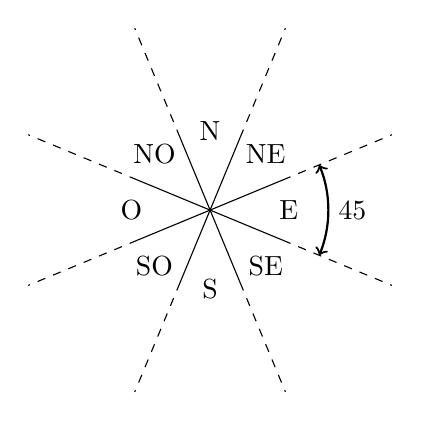
\begin{tikzpicture}
  \foreach \x/\v in {0/E,1/NE, 2/N,3/NO,4/O,5/SO,6/S,7/SE} {
    \path[draw] (0,0) -- (45*\x+22.5:1);	
    \path[draw, dashed] (45*\x+22.5:1) -- (45*\x+22.5:2.5);
    \node at (45*\x:1cm) {\v};
  }

  \path[draw, <->, thick] (22.5:1.5) arc (22.5:-22.5:1.5)
  node[pos=.5,right] {\SI{45}{\degree}};
\end{tikzpicture}
    \caption{Mosélisation des relations cardinales à l'aide d'un
      modèle conique. D'après \textcite{Renz2004}.}
  \label{fig:mod_orient_cone}
\end{figure}

\begin{figure}
  \centering
    \begin{tikzpicture}
	\begin{scope}
	\path[ffa] (-1.5,0) --++ (3,0) --++ (0,1.5) --++ (-3,0) --cycle;
	\path[ffa2] (-1.5,0) --++(3,0) --++ (0,-1.5) --++ (-3,0) -- cycle;

	\path[draw] (-1.5,0) --++ (3,0) node[pos=0.5,above]{Nord} node[pos=0.5,below]{Sud};	
	\end{scope}

	\begin{scope}[xshift=4cm]
	\path[ffa] (0,-1.5) --++ (0,3) --++ (1.5,0) --++ (0,-3) --cycle;
	\path[ffa2] (0,-1.5) --++(0,3) --++ (-1.5,0) --++ (0,-3) -- cycle;
	\path[draw] (0,-1.5) --++ (0,3) node[pos=0.5,right]{Est} node[pos=0.5,left]{Ouest};	
	\end{scope}
	\begin{scope}[xshift=8cm]
	\path[ffa] (0,-1.5) --++(0,1.5) --++ (-1.5,0) --++ (0,-1.5) -- cycle;
	\path[ffa2] (0,1.5) --++(0,-1.5) --++ (-1.5,0) --++ (0,1.5) -- cycle;
	\path[ffa] (0,1.5) --++(0,-1.5) --++ (1.5,0) --++ (0,1.5) -- cycle;
	\path[ffa2] (0,-1.5) --++(0,1.5) --++ (1.5,0) --++ (0,-1.5) -- cycle;

	\foreach \x/\v in {0/NE,90/NO, 180/SO, 270/SE}{
	\path[draw] (0,0) -- (\x:1.5);	
	\node at (\x+45:1){\v};
}

	\end{scope}
\end{tikzpicture}
  \caption{Modélisation des relations cardinales à l'aide d'un modèle
    par demi-plans. D'après \textcite{Frank1992}.}
  \label{fig:mod_orient_half}
\end{figure}


\textcite{Frank1992} propose une extension du modèle à demi-plans
définissant une zone neutre, plus adaptée aux objets d'extension
spatiale non-nulle (\autoref{fig:mod_orient_half2}).

\begin{figure}
  \centering
    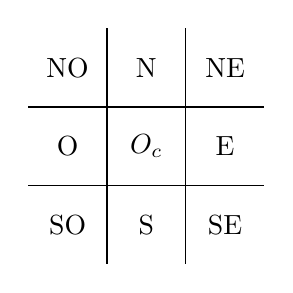
\begin{tikzpicture}

	\path[draw] (-1.5,-.5) --++ (3,0);	
	\path[draw] (-1.5,.5) --++ (3,0);
	\path[draw] (-.5,1.5) --++ (0,-3);	
	\path[draw] (.5,1.5) --++ (0,-3);	

	\foreach \x/\v in {0/E,90/N, 180/O,270/S} {
		\node at (\x:1) {\v};
}

	\foreach \x/\v in {45/NE,135/NO, 225/SO,315/SE} {
		\node at (\x:1.4142) {\v};
}
	\node at (0,0) {$\text{O}_\text{c}$};


\end{tikzpicture}
  \caption{Modèlisation des relations cardinales à l'aide d'un modèle
    par demi-plans avec une zone neutre, d'après \textcite{Frank1992}}
  \label{fig:mod_orient_half2}
\end{figure}

% Entre objets
Ces trois modèles ne permettent cependant que de définir des relations
orientationnelles cardinales et non entre deux objets, contrairement à
des modèles comme le modèle des cinq interactions de
\textcite{Clementini2006}. Ce modèle se fonde sur un principe
similaire au modèle des 9 intersections, déjà présenté. Il permet de
modèliser 5 relations projectives entre un objet à localiser et deux
autres objets servant de référence. À partir de ces deux objets, 5
zones sont définies, correspondant aux relations \emph{avant, après,
  entre, à gauche} et \emph{à droite.} En étudiant l'intersection de
ces objets avec ces cinq zones on peut construire 34 relations
différentes. Comme dans les modèles dérivés du modèle 4IM, ces
relations sont formalisées à l'aide d'une matrice, où chacune des 5
valeurs correspond à une des 5 zones définies par le modèle.

Enfin, comme pour les modèles topologiques, des extensions
tridimensionnelles de ces modèles ont été proposées.


\paragraph{Les relations d'orientation relative}

% TODO
%\tdi{Voir si c'est nécessaire de compléter}

% Définition
Les relations d'orientation relatives sont définies par
\textcite{Duchene2019} comme des relations
\enquote{concern\textins{ant} l'écart angulaire entre deux objets
  ayant une direction privilégiée d'allongement et pouvant à ce titre
  être assimilés à des segments \textelp{}}. Comme nous l'expliquions
précédemment, la phrase : \enquote{J'ai pris la première à droite}
correspond à une \emph{relation d'orientation relative.} Des modèles
spécifiques à ce type de relations ont été proposés dans la
littérature, comme les \emph{calculi} de
\textcite{Schlieder1995,Isli2000}.

\subsubsection{Les relations de visibilité}
%TODO
% \tdi{Idem, faut-il plus de détail ?}

Comme pour les \enquote{durées de déplacement}, détaillées ci-dessus,
les \enquote{relations de visibilité} ne s'expriment pas à l'aide
d'une préposition spatiale, comme \enquote{sur} ou \enquote{dans}, il
s'agit donc d'une \emph{relation de localisation,} mais pas d'une
\emph{relation spatiale.} Contrairement aux distances, où leur
expression peu prendre plusieurs formes, les \emph{relations de
  localisation visuelles} sont toujours exprimées d'une même
manière. On décrit ce qu'on a (ou pas) dans notre champ de
vision. Ainsi la spatialisation de ce type \emph{d'indice de
  localisation} nécessite de pouvoir construire le champ de visibilité
d'un objet, quelle que soit sa nature.

La question de la construction de zones de visibilités a été
longuement abordée dans le domaine des SIG, notamment en vue
d’applications pour l'étude de paysages. Mais la notion de visibilité
peut également s'appliquer à des éléments de localisation tels que :
\enquote{Je suis à l'ombre}, que l'on retrouve notamment dans le
\emph{fil rouge} (\ref{chap:1}). En effet, être, ou non, à l'ombre
revient à avoir, ou non, une relation de visibilité avec le
Soleil. Or, dans un contexte montagnard les ombres sont très présentes
à cause des reliefs, la possibilité d'identifier les zones situés au
Soleil ou à l'ombre est donc utile pour localiser des personnes
\autocite{Houpert2003}. \textcite{Sahraoui2016} distinguent deux types
d'analyses de visibilités différentes, les analyses planimétriques
\enquote{consist\textins{ant} à caractériser les relations
  d’intervisibilité entre des lieux d’observation et leur espace
  environnant \textelp{}} et les analyses tangentielles qui
\enquote{\textelp{} mesur\textins{ent} le paysage visible dans la
  rétine d’un observateur virtuel en tenant compte du développement
  vertical des objets du paysage \textelp{}}.

% Applications

\paragraph{Approche planaire}

La spatialisation d'une \emph{relation de visibilité} nécessite de
construire une zone où l'objet de référence est visible. Cette zone,
généralement qualifiée de \emph{bassin de visibilité,} est construite
à partir d'un \ac{mnt} décrivant le relief. Les algorithmes de
construction des bassins de visibilité vérifient ensuite, pour toutes
les positions de la zone étudiée, si l'objet de référence est visible,
ou non. Par conséquent les \emph{bassins de visibilité} sont
généralement binaires, on distingue les positions d'où l'on voit, de
celle où on ne voit pas.

D'autres travaux proposent de traiter les relations de visibilité de
manière multivalente, \ie en distinguant les situations où la
visibilité est partielle de celles où la visibilité est
totale. \textcite{Ramos2003} définit la notion de \emph{fenêtre de
  visibilité,} qui est la géométrie 3D englobant toutes les lignes
reliant la géométrie observée à la géométrie de l'observateur. Cette
modélisation vectorielle permet de construire l'intersection de la
fenêtre de visibilité avec le relief et le
sursol. \textcite{Ramos2003} définit 3 types de visibilité en fonction
de l'intersection de la \emph{fenêtre de visibilité.} Si elle est
entièrement visible la visibilité est totale, si elle est totalement
obstruée alors l'objet est invisible et si elle est partielle obstruée
la visibilité est partielle.

\textcite{Lonergan2014} ont, quant à eux, proposé de prendre en compte
les capacités perspectives des observateurs. En effet, dans les
approches précédemment présentées, l'observateur est modélisé par une
géométrie, sans que ces caractéristiques perspectives, comme son champ
de vision, soient prises en compte. \textcite{Lonergan2014}
définissent le concept de \emph{fenêtre de visibilité} comme un
sous-ensemble du \emph{bassin de visibilité,} duquel on aurait retiré
toutes les zones invisibles, compte-tenu des capacités perspectives de
l'observateur. Un être humain, par exemple, ne peut voir que dans une
direction donnée, et pas à 360 degrés autour de lui. La prise en
compte des capacités perspectives permet à \textcite{Lonergan2014} de
définir une typologie des relations de visibilité, distinguant, par
exemple, les moments où l'observateur se focalise sur un point (ce qui
tend à réduire son champ de vision) de ceux où il scanne le paysage
(et où l'observateur regarde dans toutes les directions autour de
lui).

\paragraph{Approche tangentielle}

D'autres travaux proposent quant à eux d'étudier les positions
relatives des objets dans le champ de vision de l'observateur.
\textcite{Santos2015} proposent une typologie des
relations de visibilité fondée sur les relations de Allen. Cette
typologie permet de décrire les relations entre deux objets, du point
de vue d'un observateur qui aurait un champ de vision de 180 degrés.
% ROC 20
\textcite{Randell2001} proposent une solution similaire avec le ROC-20
(\emph{Region Occlusion Calculus}), une formalisation des relations
topologiques entre les silhouettes des objets vus par
l'utilisateur. Ce modèle permet également de modéliser des positions
relatives entre objets vus (\eg du point de vue de l'utilisateur
l'objet \emph{a} est à gauche de \emph{b}), mais également des
relations d'occlusion relative (\eg \emph{a} cache un bout de \emph{b}
et inversement).

%%% Local Variables:
%%% mode: latex
%%% TeX-master: "../../../../main"
%%% End:
